\documentclass[12pt,a4paper,UTF8]{ctexart}
	%10pt:正文字体为12pt,缺省为10pt;各层级字体大小会根据正文字体自动调整
	%a4paper:纸张大小a4;
	%UTF8:中文要求
\usepackage{geometry}%用于设置上下左右页边距
	\geometry{left=2.5cm,right=2.5cm,top=3.2cm,bottom=2.8cm}
\usepackage{xeCJK,amsmath,paralist,enumerate,booktabs,multirow,graphicx,subfig,setspace,listings,lastpage,hyperref,setspace}
	%xeCJK:中文字体(如楷体,作者和机构需要用到)的设置
	%amsmath:数学公式
	%paralist,enumerate:自定义项目符号
	%booktabs:三线图,论文常用的表格风格
	%multirow:复杂表格
	%graphicx,float: 插入图片
	%subfig:并排排版图片、竖向排版图片
	%setspace:设置行间距等功能
	\setlength{\parindent}{2em}%正文首行缩进两个汉字
	%listings:用于排版各种代码;比如matlab的代码
	\lstset{language=Matlab}%matlab代码
	%lastpage:获取总页数;
	%hyperref:超链接,和lastpage搭配.
\usepackage{fancyhdr}
	%fancyhdr:一个很强大的宏包,用于自定义设计页面风格并命名以供调用。
	\pagestyle{fancy}
	\rhead{实验B10 单缝衍射相对光强分布}
	\lhead{基础物理实验\uppercase\expandafter{\romannumeral2}会议摘要}
	\cfoot{Page \thepage/\pageref{LastPage}}  %当前页\总页数
		%分别是右页眉、左页眉、中页脚、右页脚
	\renewcommand{\headrulewidth}{0.4pt}
	\renewcommand{\theenumi}{(\arabic{enumi})}
	\setlength\headheight{15pt}
\usepackage{longtable}

\begin{document}

%%begin-------------------标题与信息-----------------------%%

%%标题
\begin{center}
\LARGE\textbf{实验B10 单缝衍射相对光强分布}
\end{center}


%%end-------------------标题与信息-----------------------%%
\doublespacing
	\vspace{4em}
	%vspace:调整垂直空白,可以自己调整;缩小abstract和center(以及maketitle)的间距
	%\noindent %备用:摘要无缩进
	{\bf 摘{} 要:}
	{\zihao{-4} 光的衍射是光的波动性的基本特征之一,在结构测定及精确测量领域有着广泛的应用。
	本实验首先测定单缝衍射的相对光强分布。将型号为QY-10,波长为632.8nm的He-Ne激光器与狭缝、光功率测试仪的光探头和光屏等呈直线放置在光学平台上,并使其保持在同一高度。
	调整光源至狭缝距离调整为5cm,狭缝宽度为0.264mm,狭缝与光探头在X方向上的距离为86.05cm。此时主极大宽度约为5mm,各级衍射条纹清晰。
	沿Y轴移动光探头,使光功率最大,记录此时位置$x$。
	单向移动光探头,每移动0.1mm或0.2mm记录一次光功率值,直至第三次极大。
    以光探头相对移动距离为横坐标,光功率相对值为纵坐标拟合曲线,并在同一张图中作出理论曲线相比较。可以看出,实验曲线的趋势与理论公式的趋势基本一致。
	由实验曲线测得的数据进行拟合,可以得到狭缝的宽度 0.24  mm,与实验中狭缝实际宽度的相对误差为9\%。
	
	除此之外,本实验还测定单缝衍射的相对光强分布。
	光源采用GY-6型溴钨灯,摘下灯前毛玻璃,将光探头放置于光源前5cm处,每远离1cm-2cm测一次光功率。
	对光源至光探头距离平方的导数与其对应光功率作图并线性拟合,
	发现在距离钠灯一定距离时,光功率计的读数与入射光强成线性关系。因此可以说光探头工作在线性区域。}
	\par%空的新行的高度。
	\textbf{关键词}:夫琅禾费单缝衍射,光功率测试仪,曲线拟合
	\vspace{3em}

\newpage

	\renewcommand{\abstractname} {} %不显示摘要名字
	\begin{center}%
	    {\LARGE\bfseries Experiment B10: Single Slit Diffraction Relative Intensity Distribution\footnotemark[1]  \par}%
	    \vskip 1.4em%
	    {\large
	    \lineskip .75em%
	    \begin{tabular}[t]{c}%
	        \large XXX$^{1}$
	    \end{tabular}\footnotemark[2] \par
	    }%
	    \vskip 0.4em%
	    {\normalsize School of Physics, Sun Yat-sen University, Guangzhou  { \rm 510275}, China}
	\end{center}
	\begin{abstract}
		\vspace{-2em}  %缩小abstract和center(以及maketitle)的间距
	    	{\bf Abstract:}
			{The diffraction of light is one of the basic characteristics of light, which is widely used in the field of structure determination and accurate measurement.
			Firstly, the relative intensity distribution of single slit diffraction was measured.
			The QY-10 He-Ne laser with wavelength of 632.8nm was placed on the optical platform in a straight line with the slit, the optical probe of the optical power tester and the optical screen, and kept at the same height.
			We adjusted the distance between the light source and the slit to 5cm, width of the slit to 0.264mm, and the distance between the slit and the light probe in the X direction to 86.05cm.
			At this time, the diffraction patterns at all levels are clear.
			We moved the optical probe along the Y-axis to maximize the optical power and recorded the position $x$.
			Then move the optical probe in one direction and record the optical power value every 0.1mm or 0.2mm until the third peak.
			The relative moving distance of the optical probe was taken as the abscissa and the relative value of the optical power was taken as the ordinate fitting curve.
			It can be seen that the trend of the experimental curve is basically consistent with that of the theoretical formula.
			By fitting the data measured from the experimental curve, the width of the slit is 0.24   mm, and the relative error is 9\%.
			In addition, the relative intensity distribution of single slit diffraction is also measured.
			GY-6 bromotungsten lamp was used as the light source. 
			The frosted glass in front of the lamp was removed, and the light probe was placed 5cm in front of the light source. The light power was measured every time it was 1cm-2cm away.
			The derivative of the square distance from the light source to the light probe and the corresponding light power were plotted and linearly fitted.
			It is found that there is a linear relationship between the reading of the optical power meter and the incident light intensity at a certain distance from the sodium lamp.Thus the light probe can be said to operate in a linear region.}
			\par%空的新行的高度。
		\textbf{Key words}: Fraunhoffer single slit diffraction, optical power tester, curve fitting
	\end{abstract}
\footnotetext[1]{{Supported and taught by Han Shen, School of Physics, Sun Yat-sen University}}
\footnotetext[2]{{Corresponding author. E-mail:\url{morb@mail2.sysu.edu.cn}}}


\subsection*{【数据记录与处理】}
\subsubsection*{1.测定单缝衍射的相对光强分布}
实验参数:狭缝与光探头在X方向上的距离为Z=86.05cm,狭缝宽度为0.264mm,高度为2.59cm,光屏宽度15cm.

测量光强分布时,将实验测得的探头移动距离与光功率值记录,记录下光功率最大时光功率计和平移螺杆的读数,之后在X方向上平移光探头,每隔一段距离记录一次光强和光探头移动距离$\varDelta x$
,则狭缝与光探头的距离为$X=\sqrt{(Z^2+\varDelta x^2)}$,衍射角正弦值为$sinθ=\varDelta x/X$,光功率相对值$I_\theta/I_0$,相关数据列表如表1:
\begin{table}[htbp]
	\caption{光强分布相关数据}
	\centering
    \begin{longtable}{cccc}
	\toprule
	探头移动距离$\varDelta x/mm$ & 光功率$I_\theta/nW$ &$sin\theta $ &光功率相对值$I_\theta/I_0 $\\
	\midrule

	0.0&276&0.00000000&1.00000000 \\
	0.1&275&0.00011621&0.99637681 \\
	0.2&274&0.00023242&0.99275362 \\
	0.3&273&0.00034863&0.98913043 \\
	0.4&272&0.00046485&0.98550725 \\
	0.5&270&0.00058106&0.97826087 \\
	0.6&268&0.00069727&0.97101449 \\
	0.7&265&0.00081348&0.96014493 \\
	0.8&260&0.00092969&0.94202899 \\
	0.9&257&0.00104590&0.93115942 \\
	1.0&250&0.00116212&0.90579710 \\
	1.1&242&0.00127833&0.87681159 \\
	1.2&236&0.00139454&0.85507246 \\
	1.3&231&0.00151075&0.83695652 \\
	1.4&222&0.00162696&0.80434783 \\
	1.5&217&0.00174317&0.78623188 \\
	1.6&210&0.00185938&0.76086957 \\
	1.7&201&0.00197560&0.72826087 \\
	1.8&194&0.00209181&0.70289855 \\
	1.9&187&0.00220802&0.67753623 \\
	2.0&181&0.00232423&0.65579710 \\
	2.2&166&0.00255665&0.60144928 \\
	2.4&151&0.00278908&0.54710145 \\
	2.6&135&0.00302150&0.48913043 \\
	2.8&121&0.00325392&0.43840580 \\
	3.0&106&0.00348635&0.38405797 \\
	3.2&93.1&0.00371877&0.33731884 \\
	3.4&80.1&0.00395119&0.29021739 \\
	3.6&67.0&0.00418361&0.24275362 \\
	3.8&55.3&0.00441604&0.20036232 \\
	4.0&43.8&0.00464846&0.15869565 \\
	4.2&36.0&0.00488088&0.13043478 \\
	4.4&27.7&0.00511331&0.10036232 \\
	4.6&20.5&0.00534573&0.07427536 \\
	4.8&14.6&0.00557815&0.05289855 \\
	5.0&10.0&0.00581058&0.03623188 \\
	5.2&6.3&0.00604300&0.02282609 \\
	5.4&3.5&0.00627542&0.01268116 \\
	5.6&1.6&0.00650784&0.00579710 \\
	5.8&0.7&0.00674027&0.00253623 \\
	6.0&0.4&0.00697269&0.00144928 \\
	\bottomrule
\end{longtable}%
\label{tab:data1}%
\end{table}%

\begin{table}[htbp]
\centering
\begin{longtable}{cccc}
\toprule
探头移动距离$\varDelta x/mm$ & 光功率$I_\theta/nW$ &$sin\theta $ &光功率相对值$I_\theta/I_0 $\\
\midrule


	6.2&0.6&0.00720511&0.00217391 \\
	6.4&1.4&0.00743754&0.00507246 \\
	6.6&2.6&0.00766996&0.00942029 \\
	6.8&4.1&0.00790238&0.01485507 \\
	7.0&5.6&0.00813481&0.02028986 \\
	7.2&7.3&0.00836723&0.02644928 \\
	7.4&9.0&0.00859965&0.03260870 \\
	7.6&10.5&0.00883207&0.03804348 \\
	7.8&11.9&0.00906450&0.04311594 \\
	8.0&12.9&0.00929692&0.04673913 \\
	8.2&13.7&0.00952934&0.04963768 \\
	8.4&14.3&0.00976177&0.05181159 \\
	8.6&14.6&0.00999419&0.05289855 \\
	8.8&14.6&0.01022661&0.05289855 \\
	9.0&14.3&0.01045904&0.05181159 \\
	9.2&13.7&0.01069146&0.04963768 \\
	9.4&12.9&0.01092388&0.04673913 \\
	9.6&12.0&0.01115630&0.04347826 \\
	9.8&10.9&0.01138873&0.03949275 \\
	10.0&9.8&0.01162115&0.03550725 \\
	10.2&8.5&0.01185357&0.03079710 \\
	10.4&7.2&0.01208600&0.02608696 \\
	10.6&5.9&0.01231842&0.02137681 \\
	10.8&4.6&0.01255084&0.01666667 \\
	11.0&3.5&0.01278327&0.01268116 \\
	11.2&2.5&0.01301569&0.00905797 \\
	11.4&1.7&0.01324811&0.00615942 \\
	11.6&1.0&0.01348053&0.00362319 \\
	11.8&0.5&0.01371296&0.00181159 \\
	12.0&0.2&0.01394538&0.00072464 \\
	12.2&0.0&0.01417780&0.00000000 \\
	12.4&0.0&0.01441023&0.00000000 \\
	12.6&0.2&0.01464265&0.00072464 \\
	12.8&0.5&0.01487507&0.00181159 \\
	13.0&0.8&0.01510750&0.00289855 \\
	\bottomrule
\end{longtable}%
\label{tab:data1}%
\end{table}%

\begin{table}[htbp]
\centering
\begin{longtable}{cccc}
\toprule
探头移动距离$\varDelta x/mm$ & 光功率$I_\theta/nW$ &$sin\theta $ &光功率相对值$I_\theta/I_0 $\\
\midrule


	13.2&1.2&0.01533992&0.00434783 \\
	13.4&1.8&0.01557234&0.00652174 \\
	13.6&2.3&0.01580476&0.00833333 \\
	13.8&2.8&0.01603719&0.01014493 \\
	14.0&3.4&0.01626961&0.01231884 \\
	14.2&3.8&0.01650203&0.01376812 \\
	14.4&4.3&0.01673446&0.01557971 \\
	14.6&4.6&0.01696688&0.01666667 \\
	14.8&4.9&0.01719930&0.01775362 \\
	15.0&5.0&0.01743173&0.01811594 \\
	15.2&5.2&0.01766415&0.01884058 \\
	15.4&5.1&0.01789657&0.01847826 \\
	15.6&4.9&0.01812899&0.01775362 \\
	15.8&4.7&0.01836142&0.01702899 \\
	16.0&4.4&0.01859384&0.01594203 \\
	16.2&4.0&0.01882626&0.01449275 \\
	16.4&3.6&0.01905869&0.01304348 \\
	16.6&3.1&0.01929111&0.01123188 \\
	16.8&2.7&0.01952353&0.00978261 \\
	17.0&2.2&0.01975596&0.00797101 \\
	17.2&1.8&0.01998838&0.00652174 \\
	17.4&1.3&0.02022080&0.00471014 \\
	17.6&0.9&0.02045322&0.00326087 \\
	17.8&0.6&0.02068565&0.00217391 \\
	18.0&0.4&0.02091807&0.00144928 \\
	18.2&0.2&0.02115049&0.00072464 \\
	18.4&0.1&0.02138292&0.00036232 \\
	18.6&0.0&0.02161534&0.00000000 \\
	18.8&0.0&0.02184776&0.00000000 \\
	\bottomrule
	\end{longtable}%
	\label{tab:data2}%
\end{table}%

以$sin\theta$为横坐标,光功率相对值$I_\theta/I_0$为纵坐标作图,并在同一张图中,自定义拟合曲线如图三:

\begin{equation*}
	\frac{I_{\theta}}{I_0}={\left(\frac{sin(\frac {\pi ax}{\lambda})}{\frac{\pi ax}{\lambda}}\right)}^2
\end{equation*}

\begin{figure}[htbp]
	\caption{曲线拟合}
	\centering
	\includegraphics[width=0.8\textwidth]{img//reg1.jpg}
	\label{fig:9}
\end{figure}

对实验参数做仿真,结果见图一,图二:

\begin{figure}[htbp]
	\caption{仿真界面}
	\centering
	\includegraphics[width=\textwidth]{img//im.jpg}
	\label{fig:5}
\end{figure}
\begin{figure}[htbp]
	\caption{仿真结果}
	\centering
	\includegraphics[width=0.8\textwidth]{img//re.jpg}
	\label{fig:4}
\end{figure}

代入实验参数可以计算出理论狭缝宽度为0.24mm,将各主极大与仿真值对比,见表5:
\begin{table}[htbp]
	\caption{实验各极大与仿真值比较}
	\centering
    \begin{tabular}{cccc}
	\toprule
	极大的级数&理论$I_\theta/I_0$&实验$I_\theta/I_0$&相对误差\\
	\midrule
	主极大&1&1&0\\
    第一次极大&0.0469&	0.0529& 12.7\%\\
    第二次极大&0.0166&	0.0188& 13.2\%\\
    \bottomrule
	\end{tabular}%
	\label{tab:data2}%
\end{table}%




\subsubsection*{2. 检测光功率计的读数与入射光强的线性关系}

a为参数,进行拟合,同时取$a=2.29×10^{-4}$ m将理论公式下的曲线在同一张图中画出,最终得到拟合曲线与理论曲线如图四。

在实验2中,测得起始位置光源与光探头距离为$Z_0=22.0cm$,而后以2cm的间隔测量至40cm,之后以4cm的间隔测量至80cm,最后以5cm的间隔测量至100cm.实验数据列表如下。

\begin{table}[htbp]
	\caption{光度计读数与距离相关数据}
	\centering
    \begin{tabular}{cccccc}
	\toprule
	Z/cm & $1/Z^2/cm^{-2}$&	P/nW & Z/cm	& $1/Z^2/cm^{-2}$&	P/nW\\
	\midrule
    5&0.04&492&16&0.00390625&66.0\\
	6&0.02777778&384&18&0.00308641&47.4\\
	7&0.02040816&304&20&0.0025&38.1\\
	8&0.015625&245&22&0.00206611&37.1\\
	9&0.01234568&198.2&24&0.00173611&30.7\\
	10&0.01&146.2&26&0.00147929&26.1\\
	12&0.0069444&101.1&28&0.00127551&21.0\\
	14&0.0051020&82.6&30&0.00111111&19.9\\
	\bottomrule
	\end{tabular}%
	\label{tab:data2}%
\end{table}%

作光功率P关于距离平方倒数的图像并进行定截距拟合,截距为零。

\begin{figure}[htbp]
	\caption{线性拟合}
	\centering
	\includegraphics[width=0.8\textwidth]{img//reg2.png}
	\label{fig:6}
\end{figure}





其中,$R^2=0.98692$,说明两者线性关系极强,可认为光探头工作在线性区.


\subsection*{【误差分析】}
\subsubsection*{1. 测定单缝衍射的相对光强分布}
\begin{enumerate}
	\item	实验测得的数据点不够多,分步值仍不够小,不能保证光强出现极大时的数据被测量到,这会导致光强极大点被跳过,进而导致极大的误差
    \item   受困于仪器的极限,主极大不可能测得完全准确,会对后续计算差生误差。
    \item   实验中不能保证完全的无光环境,会使光探头产生一定的误差。
    \item   在读数时,即使没有干扰实验仪器,光探头读数也在不断变化,在估读的过程中会差生误差。
\end{enumerate}
\subsubsection*{2.检测光功率计的读数与入射光强的线性关系}
\begin{enumerate}
	\item 	移动光探头时,光探头的位置不能完全摆放正确,这将导致Z值有较大的误差。
	\item 在每个位置读数前微调光探头位置的操作中可能导致人为误差。
\end{enumerate}

\subsubsection*{【结论】}
	在一定的误差范围内,可以验证单缝夫琅禾费衍射的相对光强分布与理论基本一致,并可由此求得狭缝的宽度,与实测的结果误差不大。为进一步减小误差,可考虑进一步减小步长值进行测量。
	光功率计的读数与入射光强有极强的线性关系,可以认为光探头工作在线性区。


\newpage
\subsection*{【思考题】}

\subsubsection*{1.当缝宽增加一倍,衍射花样的光强和条纹的宽度将会怎样改变?如缝宽减半,情况如何?}
答:(1)当缝宽增加一倍时,由光强分布公式可知,当缝宽增加一倍时,光强增加。条纹宽度可以根据主极大两侧暗纹之间的角距离∆θ=2λ/a来判断,角距离变为原来的一半,条纹的宽度变为原来的一半。

(2)当缝宽减半时,光强减小,角距离变为原来的两倍,条纹的宽度变为原来的两倍。

\subsubsection*{2.使用光功率计应注意那些问题?光功率计进光狭缝的宽度对实验结果有何影响?}
答:(1)使用光功率计应注意使用的光功率计的测试范围,选择适合实验需要的功率,注意选择和发射光源一样的波长,
	注意仪器在长时间闲置后,需使用仪器的自校准功能,
	注意测量时要注意保证探头与其他光学仪器共轴和减少环境光的影响。

(2)光功率计测量的是光在单位时间内所做的功,进光狭缝的宽度过大会导致沿X方向测量范围过大,不够精确,影响实验结果,狭缝太窄会导致光探头很难保持与光纤在同一直线,稍微偏离测量值就会变为零,也不准确。

\subsubsection*{3.检查光功率计探头是否工作在线性区时,能否用激光光源?}
答:不能。光强与光源的距离平方倒数成正比是球面波的特点;而激光更接近平面波,光强基本不随与光源距离而改变,不易测得光功率与距离的变化关系。

\subsubsection*{4.证明本实验能满足夫琅和费衍射条件。}

\begin{figure}[htbp]
	\centering
	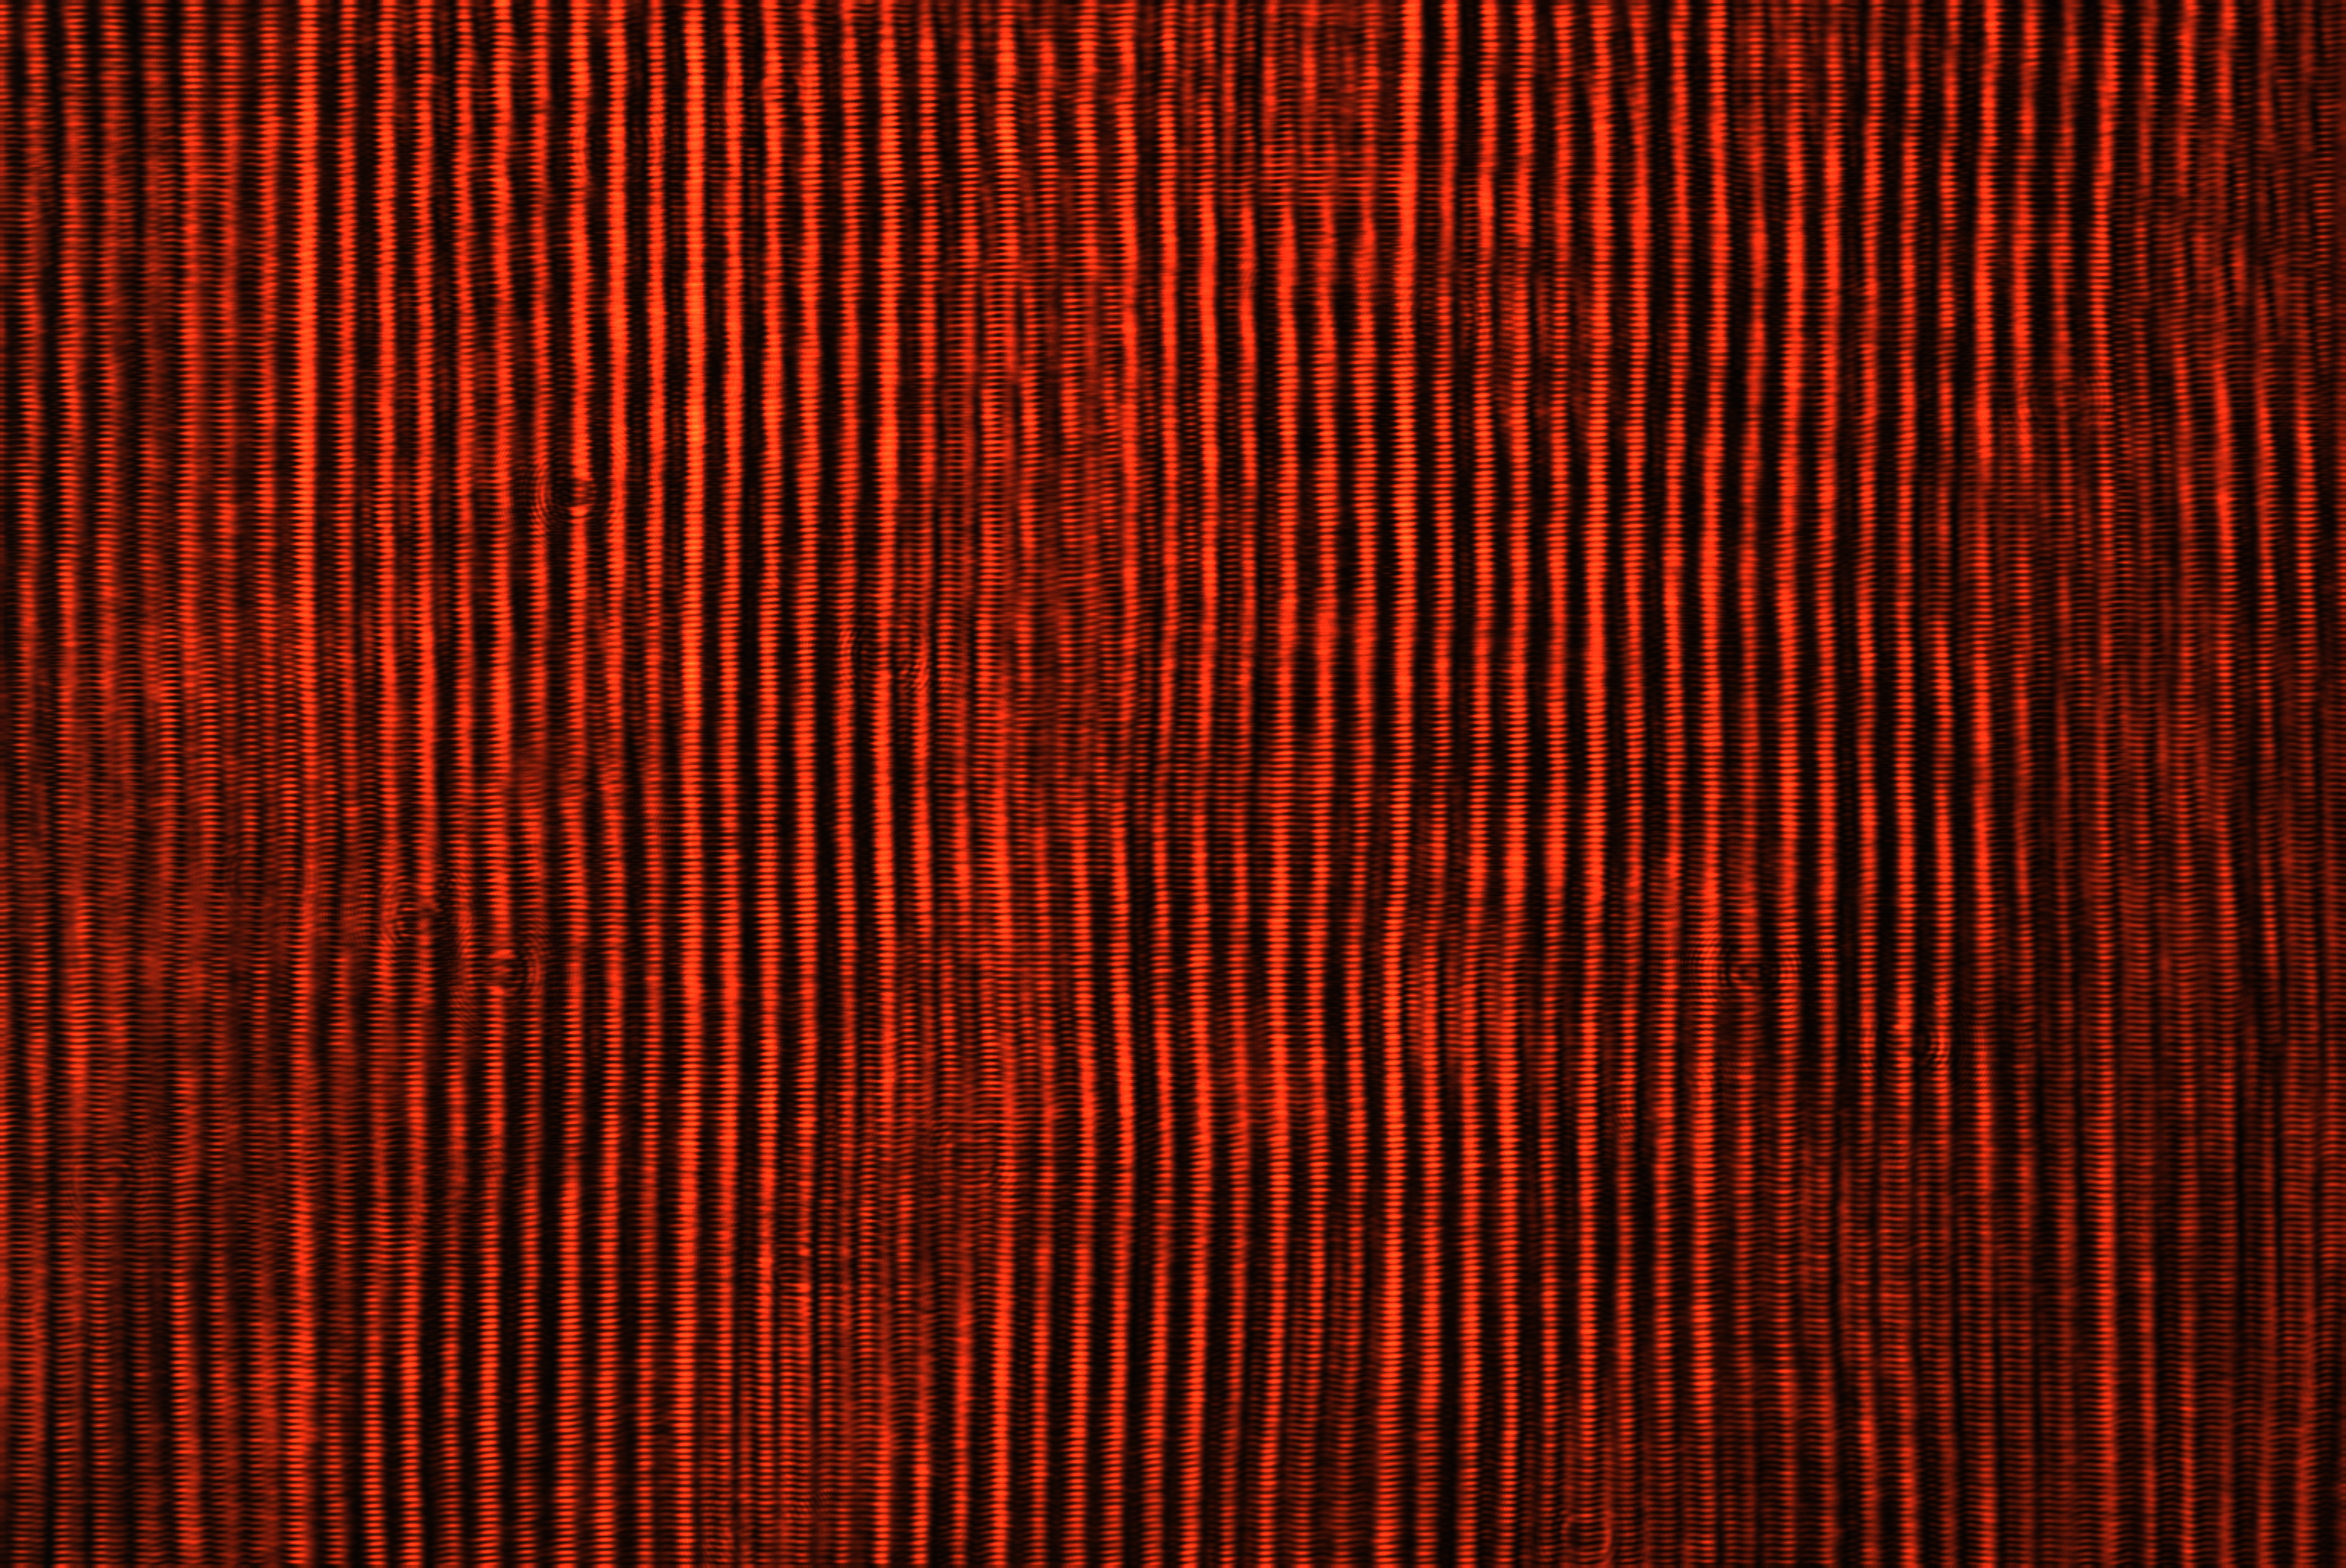
\includegraphics[width=0.6\textwidth]{img//1.png}
	\label{fig:7}
\end{figure}

证明:如图,$P_0$为衍射角$\theta=0$的一点,对于夫琅禾费衍射来说,要求缝上各点发出的次波到$P_0$时均有相同的光程,显然,只有把屏移到无穷远才能满足。
实际上,只要$AP_0$与$OP_0$的差远远小于一个波长$\lambda$,就可以满足条件。
$AP_0-OP_0=\sqrt{Z^2+(a/2)^2}-Z \ll \lambda$
因$Z\gg a$,可得

\begin{equation*}
	\sqrt{Z^2+(\frac{a}{2})^2}-Z = \frac{a^2}{8Z}
\end{equation*}

即有
$a^2 \ll 8Z \lambda$
在实验中,,λ=632.8nm,缝宽a=0.264mm,Z=89.05cm,代入后,符合上式。 

\subsubsection*{5.采用数值计算的方法画出单缝、双缝、三缝、四缝、多缝、透射光栅的相对光强分布曲线。}
答: 单缝、双缝、三缝、四缝、多缝可以看做是透射光栅的特殊情况,多缝衍射强度分布为单缝衍射光强分布与多缝干涉光强分布的相互作用结果。其表达式为:
\begin{equation*}
	I_θ=I_0^2{\left(\frac{sin(\frac {\pi a sin\theta}{\lambda})}{\frac{\pi asin\theta}{\lambda}}\right)}^2{\left(\frac{sin(N \frac {\pi d sin\theta}{\lambda})}{\frac{\pi d sin\theta}{\lambda}}\right)}^2
\end{equation*}
将a=d/2=0.264mm,N=1,2,3,4,10,100分别代入,作图如下:

\begin{figure}[htbp]
	\centering
	\subfloat[N=1]{\label{fig:8.1}
	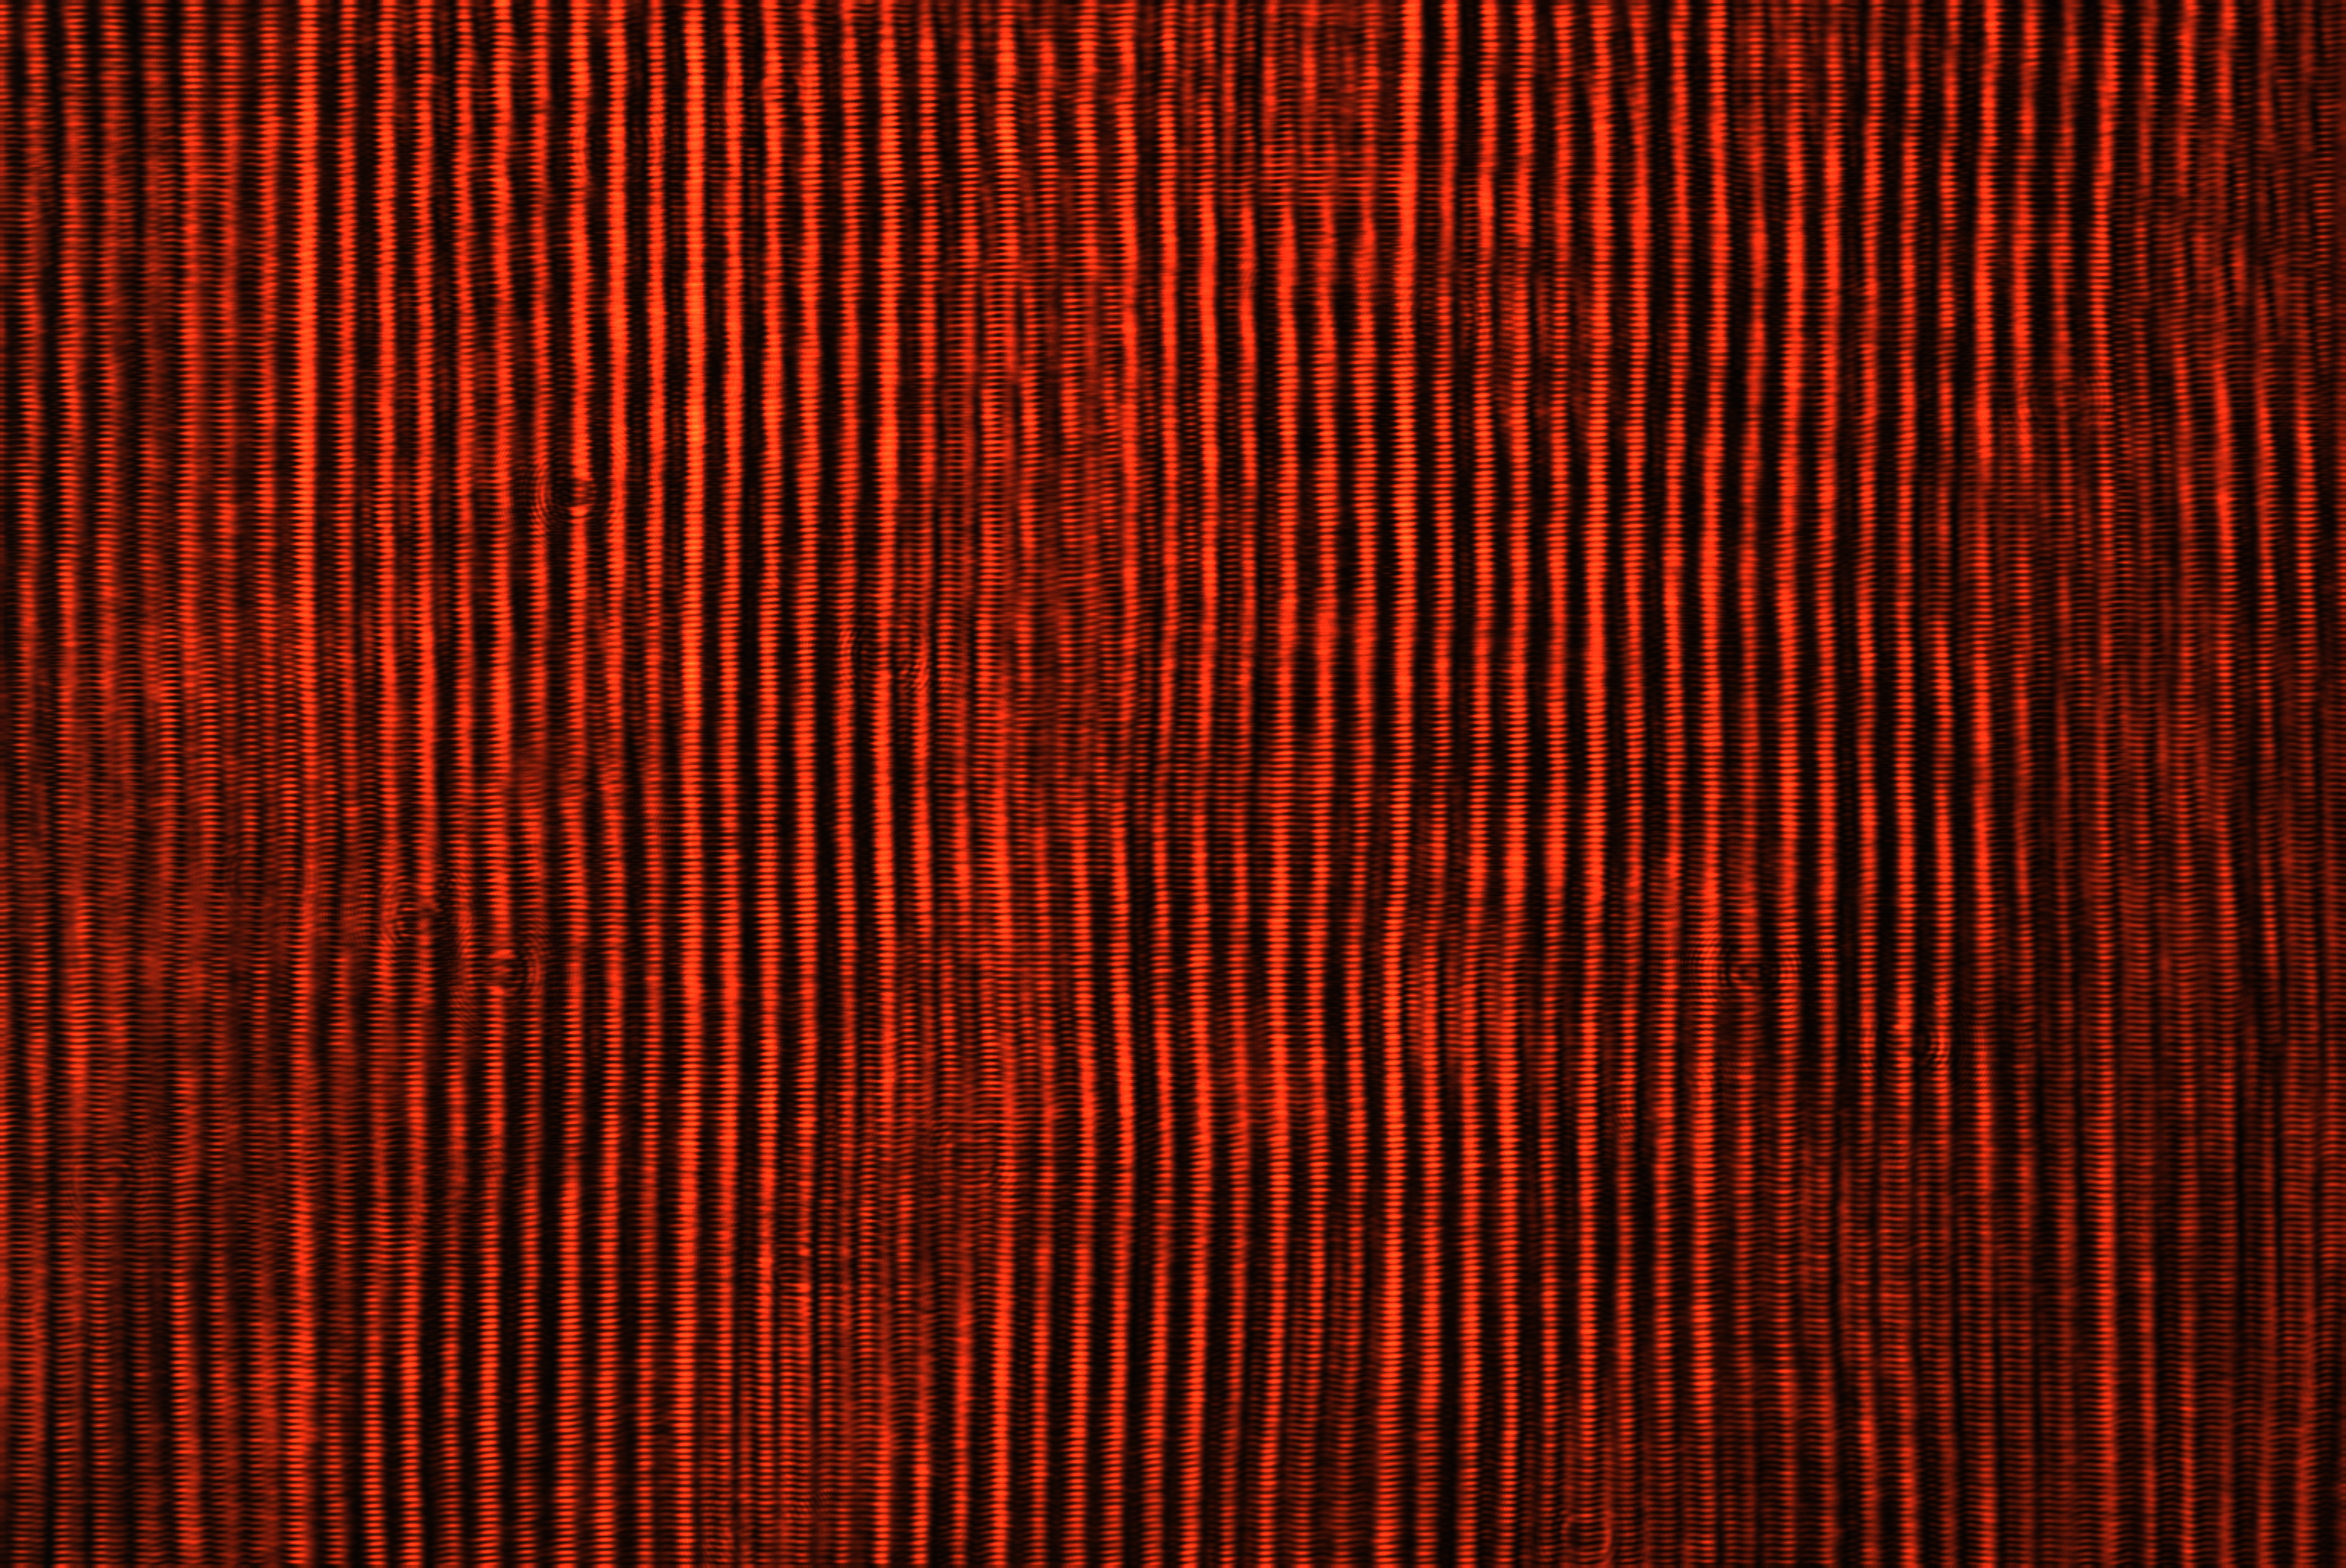
\includegraphics[width=0.33\textwidth]{img//1.jpg}
	}
	\subfloat[N=2]{\label{fig:8.2}
	\includegraphics[width=0.33\textwidth]{img//2.jpg}
	}
	\subfloat[N=3]{\label{fig:8.3}
	\includegraphics[width=0.33\textwidth]{img//3.jpg}
	}

	\subfloat[N=4]{\label{fig:8.4}
	\includegraphics[width=0.33\textwidth]{img//4.jpg}
	}
	\subfloat[N=5]{\label{fig:8.5}
	\includegraphics[width=0.33\textwidth]{img//10.jpg}
	}
	\subfloat[N=5]{\label{fig:8.6}
	\includegraphics[width=0.33\textwidth]{img//100.jpg}
	}
	\label{fig:8}
\end{figure}


\end{document}
